\chapter{Packages}

\section{Overview}
	\begin{figure}[ht]
			\begin{center}
				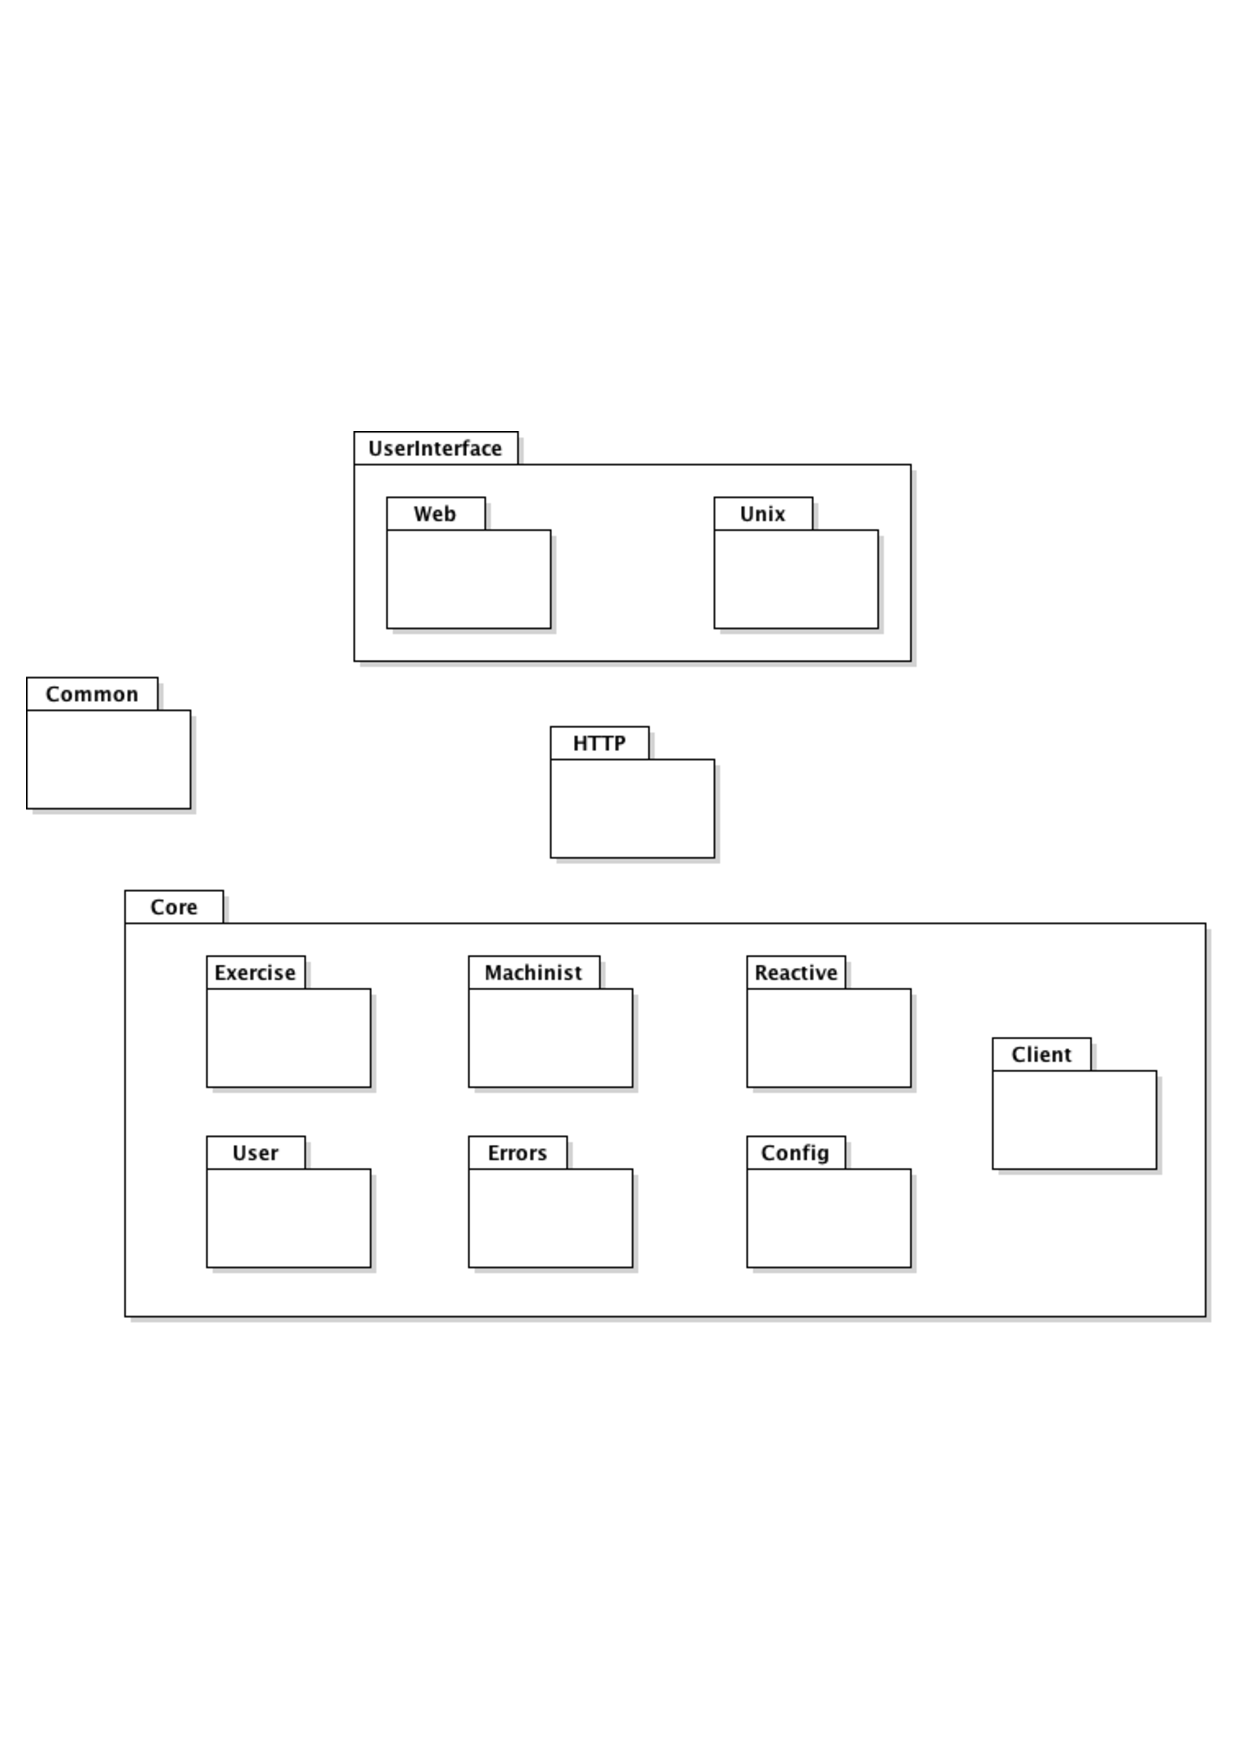
\includegraphics[width=\textwidth,  trim=2cm 12cm 2cm 1cm]{UML_figure/DP/general/DP_General.pdf}
				\caption{Diagram package : Overview}
			\end{center}
	\end{figure}
	\newpage
	\subsection{User Interface}
		This package provides every user interface components.
		\subsubsection{Web}
			This package contains the web user interface.
		\subsubsection{Text-based}
			This package contains the text-based user interface.\\
			This interface interacts with unix-like batch tools.
	\subsection{HTTP}
		This package provides the web services which allow user interfaces to communicate with the core.
	\subsection{Core}
		This package provides the core features of the system i-e. the dojo logic and the machinist to make it works.
		\subsubsection{Dojo Logic}
			This package provides the business logic (online teaching system).
		\subsubsection{Machinist}
			This package provides modules which manage sandboxed environment.
		\subsubsection{Reactive}
			This package provides modules for data update through dependencies.
		\subsubsection{VFS}
			This package provides modules for managing the sources.
	\subsection{Common}
		This package provides utilities useful for every layers of the system.
%end chapter diagram package
